\chapter{站线接触网平面设计}

\section{接触网平面设计的基本要求}
接触网平面图由平面图、表格栏、主要工程数量及材料设备表、设计说明、图标五大部分组成。接触网平面图图框示意如\ref{fig:接触网图图框示意图}所示。
% TODO: \usepackage{graphicx} required
\begin{figure}[H]
	\centering
	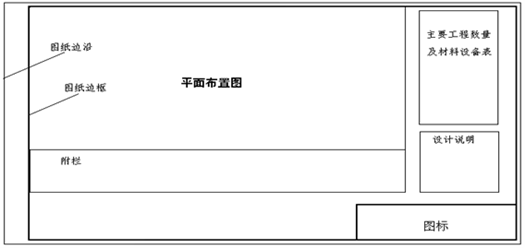
\includegraphics[width=0.7\linewidth]{figures/接触网图图框示意图}
	\caption{接触网图图框示意图}
	\label{fig:接触网图图框示意图}
\end{figure}
平面图是指用电气化铁道图形符号来表示接触网设备和结构的平面布置图,具体描述了接触网的技术参数、技术性能、设备安装位置,是接触网结构、设备、计算、平面图绘制等知识的综合应用,是接触网设计的主要技术原则的具体体现,是接触网施工、运营和维修的主要技术依据。一般根据线路平面图按1:1000或1:2000的比例绘制,图纸横向一般为3\#或4\#图宽幅,长度根据实际需要而定。

表格栏位于图纸下方,内容包括支柱侧面限界、支柱类型、地质条件、基础类型、软横跨节点、安装图号、附加导线的安装高度和图号等技术数据。表格栏中每一组技术数据对应着一根支柱或一个定位点。

工程数量统计表位于平面图的右上角,表中应注明主要设备、线材、部件及构件的数量、规格、型号。

设计说明是在进行接触网平面设计时,用以附注一些无法用图形符号表达或不易标注清楚的内容。一张完整的接触网平面图上不允许有似是而非或不确定的问题。

接触网平面图中的图标用于标明图纸的重要程度。一号图标用于首页图纸及重要的图纸;二号图标用于除一号图标外的其它图纸。图标内字体使用仿宋体,单位名称、工程名称及图名字体高度为6~8mm,其余字体高度均为4mm,字体高度与宽度的比例一般为1:0.7。

\section{支柱布置}
站场支柱布置应从站场两端咽喉区开始,首先确定道岔柱的位置,然后从站场两端道岔集中的地段开始向车站中心布置,最后完成站场咽喉区外侧道岔支柱的布置。

道岔柱的最佳位置在线间距500mm$\sim$700mm范围内,此时道岔柱与道岔理论岔心距离如\ref{tab:道岔柱与道岔理论中心的相对位置(mm)}所示。
% Please add the following required packages to your document preamble:
% \usepackage{multirow}
% \usepackage{graphicx}
\begin{table}[H]
	\centering
	\caption{道岔柱与道岔理论中心的相对位置(mm)}
	\label{tab:道岔柱与道岔理论中心的相对位置(mm)}

		\begin{tabular}{|l|l|l|l|l|l|}
			\hline
			\multirow{2}{*}{\begin{tabular}[c]{@{}l@{}}线间距\\ 道岔型号\end{tabular}} &
			\multirow{2}{*}{700} &
			\multirow{2}{*}{650} &
			\multirow{2}{*}{600} &
			\multirow{2}{*}{550} &
			\multirow{2}{*}{500} \\
			&       &       &       &       &      \\ \hline
			1/8  & 4960  & 4370  & 3780  & 3180  & 2500 \\ \hline
			1/9  & 5640  & 5070  & 4350  & 3670  & 2970 \\ \hline
			1/10 & 6200  & 5490  & 4690  & 4000  & 3200 \\ \hline
			1/11 & 6750  & 5980  & 5170  & 4310  & 3420 \\ \hline
			1/12 & 7500  & 6030  & 5720  & 4840  & 3870 \\ \hline
			1/18 & 11270 & 10050 & 8790  & 7470  & 6080 \\ \hline
			1/38 & 20740 & 18060 & 15300 & 12440 & 9480 \\ \hline
		\end{tabular}%
	
\end{table}

布置支柱时应注意以下几点:

(1)支柱位置应尽量避开风雨棚、站房、仓库、跨线桥、涵洞、信号机等建筑物,站台上尽量少设支柱,站内重要房舍(如值班室)旁的支柱不得正对门窗,站房两边支柱应尽量对称。

(2)位于两股道中间的支柱必须保证两侧限界的要求,对于站内远期预留的电化股道,应对其支柱容量和侧面限界留有余量,但单线腕臂柱的位置和容量可不考虑预留。

(3)设计下锚支柱位置时,应考虑下锚拉线的安设位置,即在支柱后10 m范围内不得有影响拉线安装的任何障碍物。

(4)终端支柱距车挡不宜小于10 m,地形受限时可设于线路的一侧。

(5)单线区段支柱应尽量设置在信号机的异侧;直线区段,位于进站信号机和区间信号机显示前方且与信号机同侧的支柱,其侧面限界应适当加大;曲线区段支柱应设置在信号机前方5m以外。

(6)在绝缘锚段关节处,为方便连接跳线,装有隔离开关的转换柱与锚柱应同侧布置。
 
(7)支柱编号,当支柱位置确定后,需给每一根支柱编号,其编排原则是:顺着公里标方向,从上行到下行先左侧后右侧的顺序编号;在复线区段下行线侧采用单数,上行线侧采用双数。

\section{拉出值大小及方向的确定}

接触线拉出值的确定从道岔较集中的区域开始,对于大站,则应在咽喉区的道岔处画出局部经放大后的接触悬挂路径图(咽喉区放大图),明确相邻道岔接触线拉出值和线岔分布情况。选定拉出值时,应保证在最大风负载作用下,跨距中任一点接触线的最大风偏移值不超过技术要求。对于道岔连接曲线上的拉出值,在选定后应进行接触线风偏移校验,当超过设计要求时,在线路条件允许的情况下可增设定位柱。

设置拉出值时应遵循以下基本原则:

(1)从咽喉区向站场中心布置,若最后遇到两相邻定位点拉出值方向相同时,可找一小跨距将其拉出值设定为零;

(2)对于同一组软横跨上的各组悬挂其拉出值方向应间隔相反,以减少软横跨支柱的受力;

(3)在标准定位的道岔柱处,两支接触线的拉出值应相等,均为375mm。且两接触线定位点的距离为100至150mm。

(4)在道岔附带曲线未端处的支柱,其拉出值一般取为400mm,通常不应小于300mm。

(5)选定拉出值时,应保证在最大风负载作用下,跨距中任一点接触线的最大风偏移值不超过技术要求(一般取为450mm)。对于道岔连接曲线上的拉出值,在选定后应进行接触线风偏移校验,当不能满足技术要求时,在线路条件允许的情况下可增设定位柱加以解决。

(6)低速道岔柱上允许不定位,但定位点两侧接触线应为自然直线状,如非工作支离股道中心较远时,要注意不使腕臂和定位器加得太长。

(7)其它如接触线高度,结构高度,支柱侧面限界等参数可参照设规的规定和前面的介绍经计算后确定。

\section{锚段关节及锚段划分}
根据站场的长度和最大锚段长度确定需要划分几个锚段以及锚段关节的大致位置。区间的锚段划分应根据线路条件和最大锚段长度确定,一些桥、遂较多地段,避免锚段关节设在隧道口、桥头。锚段走向主要针对站场存在多股接触悬挂情况(尤其在咽喉区),需理清每一支接触悬挂的走向,确定每一支接触悬挂的两端下锚位置并标示出来。

划分锚段注意事项:

(1)锚段关节不能设于道岔区;

(2)中心锚结一般设在锚段中部,原则上要求两边张力差相等;

(3)原则上一个股道一个锚段;对于较长的正线可设为一个半或两个锚段,但两锚段在站内衔接处应设为三跨非绝缘锚段关节;

(4)对于不长的站线、货线、渡线应尽量合并到别的锚段中去,不得已时也可自成一个锚段。高速线路的正线要独立设段并保证其接触悬挂的独立性,不允许与站线相交;

(5)合理确定锚段走向,应使锚段横向穿越的股道数最少,应尽量避免悬挂的二次交叉;

(6)为避免二次交叉,两组接触悬挂在通过相邻两道岔时可平行布置。
本课程设计站线锚段关节设计如\ref{fig:站线锚段关节}所示。
% TODO: \usepackage{graphicx} required
\begin{figure}[H]
	\centering
	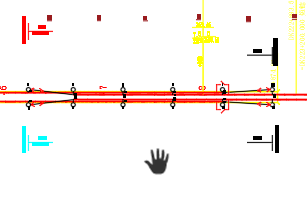
\includegraphics[width=0.7\linewidth]{figures/站线锚段关节}
	\caption{站线锚段关节}
	\label{fig:站线锚段关节}
\end{figure}

\section{咽喉区放大图}
在确定完锚段及其走向后,应绘制站场咽喉区放大图,如图3-4所示。绘制咽喉区放大图应遵循以下基本原则:

(1)放大图在纵向上保持与平面图一样的比例关系,横向比例增大为两倍;或在平面图的基础上将横向线间距加大为 ;

(2)咽喉区放大图应从靠近站场中心的道岔开始,从两侧站线做起,逐步向区间衔接处绘制,保持正线与区间衔接;

(3)为保证道岔交叉布置的定位,避开二次交叉,允许两组悬挂在同一跨距内平行等高布置;

(4)应保证两组悬挂的交叉点位于定位点与辙岔之间;

(5)放大图应明确标明锚段(股道)编号、长度及下锚位置;

(6)对于无交差布置的高速线路,应明确标出定位柱位置和相应的无交岔布置标志。

本课程设计站线咽喉区放大图设计如\ref{fig:站线咽喉放大图}所示
% TODO: \usepackage{graphicx} required
\begin{figure}[H]
	\centering
	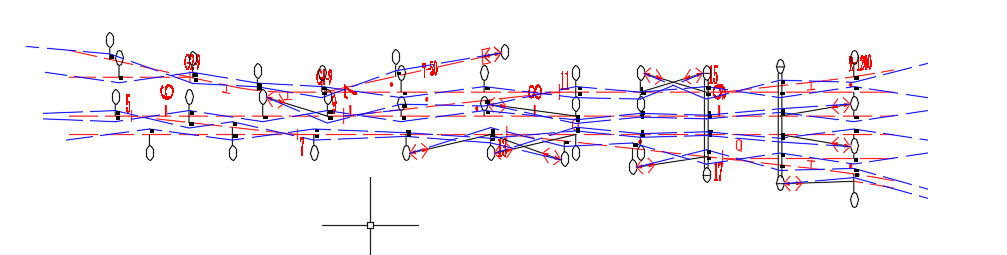
\includegraphics[width=0.7\linewidth]{figures/站线咽喉放大图}
	\caption{站线咽喉放大图}
	\label{fig:站线咽喉放大图}
\end{figure}

\section{接触网分段}
根据上述分析讨论,在本课程设计中通过锚段关节将接触网划分为五个供电分区,结合咽喉区放大图设计,该站线接触网的CAD设计图如\ref{fig:站线接触网设计图}所示。
% TODO: \usepackage{graphicx} required
\begin{figure}[H]
	\centering
	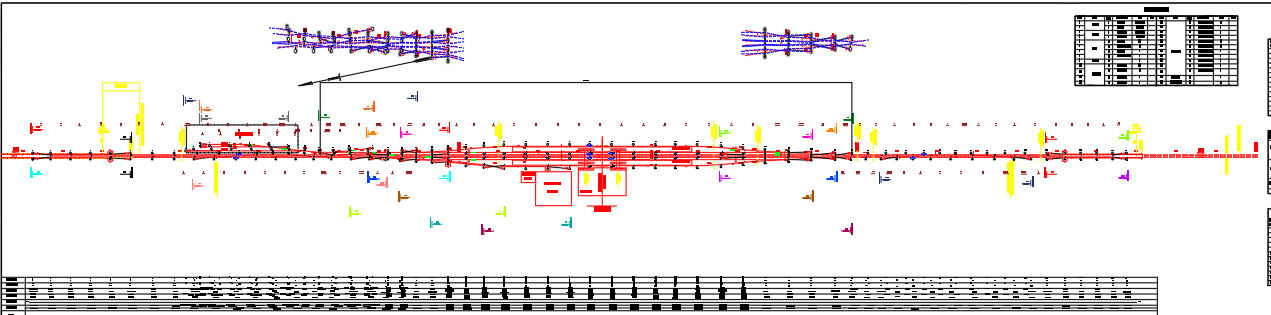
\includegraphics[width=0.7\linewidth]{figures/站线接触网设计图}
	\caption{站线接触网设计图}
	\label{fig:站线接触网设计图}
\end{figure}

\section{支柱编号及锚段标注}
支柱编号遵循了一套明确的规则,主要涉及到站场、区间、隧道、以及站场吊柱等独立单元的顺序编号。以下是对支柱编号原则的总结:支柱编号以站场、区间、隧道、站场吊柱为独立单元进行顺序编号,每个单元都有一个独立的编号体系。接触网支柱编号按照本线路从小里程侧第一根支柱开始向大里程侧进行编号。这确保了支柱的编号顺序与线路的里程方向一致。对于每个编制单元的支柱,如果编号达不到该单元最大数字位时,使用0进行前导补充。这有助于维持支柱编号的一致性和规范性。对于每个编制单元的支柱,如果编号不足两位数时,应补足成两位数。这样的规范确保了编号的一致性和易读性。举例说明:如果某站场吊柱的最大支柱编号是99,而实际编号是1,则补足前导0,编号为01。这一套支柱编号原则有助于在整个系统中建立有序、易于理解的标识体系,方便对接触网支柱进行准确定位和管理。
\section{支柱侧面限界及型号选择}

软横跨支柱限界一般为3米,在站台处为5米,位于基本站台或中间站台上的支柱,其线路侧内缘到站台边缘的距离不得小于1.5m,一般采用软横跨支柱,只在跨越四股道及以下的小站上采用钢筋混凝土支柱。软横跨由两棵支柱构成一跨式,最多跨越的股道数不超过8道,超过8道时采用两跨或三跨式。软横跨根据跨越的股道数目的不同,一般采用13m或15m钢柱,它承担着接触悬挂及支持装置的全部负荷。\ref{tab:钢支柱基础选用表}为钢支柱基础选用表。\ref{tab:独立下锚钢支柱基础选用表}。

\begin{longtable}[c]{|p{1.5cm}|p{1cm}|p{1cm}|p{1cm}|p{1cm}|p{1cm}|p{1cm}|p{1cm}|}
	\caption{钢支柱基础选用表}
	\label{tab:钢支柱基础选用表}\\
	\hline
	\multicolumn{1}{|l|}{\multirow{3}{*}{支柱类型}} &
	\multicolumn{4}{l|}{挖方及不挖不填} &
	\multicolumn{3}{l|}{填  方} \\ \cline{2-8} 
	\multicolumn{1}{|l|}{} &
	\multicolumn{4}{l|}{地质承载力(kPa)} &
	\multicolumn{3}{l|}{地质承载力(kPa)} \\ \cline{2-8} 
	\multicolumn{1}{|l|}{} &
	\multicolumn{1}{l|}{100} &
	\multicolumn{1}{l|}{150} &
	\multicolumn{1}{l|}{200} &
	\multicolumn{1}{l|}{250} &
	\multicolumn{1}{l|}{100} &
	\multicolumn{1}{l|}{150} &
	200 \\ \hline
	\endfirsthead
	%
	\endhead
	%
	\multicolumn{8}{|c|}{\textbf{8.5$\sim$10m高支柱}} \\ \hline
	\multicolumn{1}{|p{2cm}|}{G50/8.5,G50/9,G50/9.5,G50/10} &
	\multicolumn{1}{l|}{J9-5-24} &
	\multicolumn{1}{l|}{J9-2-24} &
	\multicolumn{1}{l|}{J9-1-24} &
	\multicolumn{1}{l|}{J9-1-24} &
	\multicolumn{1}{l|}{J9-6-24} &
	\multicolumn{1}{l|}{J9-4-24} &
	J9-2-24 \\ \hline
	\multicolumn{1}{|p{2cm}|}{G70/8.5,G70/9,G70/9.5,G70/10} &
	\multicolumn{1}{l|}{J9-6-30} &
	\multicolumn{1}{l|}{J9-4-30} &
	\multicolumn{1}{l|}{J9-2-30} &
	\multicolumn{1}{l|}{J9-2-30} &
	\multicolumn{1}{l|}{J9-7-30} &
	\multicolumn{1}{l|}{J9-5-30} &
	J9-3-30 \\ \hline
	\multicolumn{1}{|p{2cm}|}{G100/8.5,G100/9,G1009.5,G100/10} &
	\multicolumn{1}{l|}{J9-7-36} &
	\multicolumn{1}{l|}{J9-6-36} &
	\multicolumn{1}{l|}{J9-4-36} &
	\multicolumn{1}{l|}{J9-3-36} &
	\multicolumn{1}{l|}{J9-8-36} &
	\multicolumn{1}{l|}{J9-7-36} &
	J9-5-36 \\ \hline
	\multicolumn{1}{|l|}{G150/13} &
	\multicolumn{1}{l|}{J13-5-24} &
	\multicolumn{1}{l|}{J13-3-24} &
	\multicolumn{1}{l|}{J13-3-24} &
	\multicolumn{1}{l|}{J13-1-24} &
	\multicolumn{1}{l|}{J13-7-24} &
	\multicolumn{1}{l|}{J13-3-24} &
	J13-3-24 \\ \hline
	\multicolumn{8}{|c|}{\textbf{13m高支柱}} \\ \hline
	\multicolumn{1}{|l|}{G200/13} &
	\multicolumn{1}{l|}{J13-8-30} &
	\multicolumn{1}{l|}{J13-4-30} &
	\multicolumn{1}{l|}{J13-4-30} &
	\multicolumn{1}{l|}{J13-2-30} &
	\multicolumn{1}{l|}{J13-9-30} &
	\multicolumn{1}{l|}{J13-6-30} &
	J13-4-30 \\ \hline
	\multicolumn{1}{|l|}{GM150-250/13} &
	\multicolumn{1}{l|}{J13-7-24} &
	\multicolumn{1}{l|}{J13-5-24} &
	\multicolumn{1}{l|}{J13-3-24} &
	\multicolumn{1}{l|}{J13-1-24} &
	\multicolumn{1}{l|}{J13-7-24} &
	\multicolumn{1}{l|}{J13-5-24} &
	J13-3-24 \\ \hline
	\multicolumn{1}{|l|}{G250/13、} &
	\multicolumn{1}{l|}{\multirow{2}{*}{J13-9-30}} &
	\multicolumn{1}{l|}{\multirow{2}{*}{J13-6-30}} &
	\multicolumn{1}{l|}{\multirow{2}{*}{J13-4-30}} &
	\multicolumn{1}{l|}{\multirow{2}{*}{J13-2-30}} &
	\multicolumn{1}{l|}{\multirow{2}{*}{J13-9-30}} &
	\multicolumn{1}{l|}{\multirow{2}{*}{J13-6-30}} &
	\multirow{2}{*}{J13-6-30} \\ \cline{1-1}
	\multicolumn{1}{|l|}{GM150-250/13} &
	\multicolumn{1}{l|}{} &
	\multicolumn{1}{l|}{} &
	\multicolumn{1}{l|}{} &
	\multicolumn{1}{l|}{} &
	\multicolumn{1}{l|}{} &
	\multicolumn{1}{l|}{} &
	\\ \hline
	\multicolumn{1}{|l|}{Gs150/13} &
	\multicolumn{1}{l|}{J13-5-24} &
	\multicolumn{1}{l|}{J13-3-24} &
	\multicolumn{1}{l|}{J13-3-24} &
	\multicolumn{1}{l|}{J13-1-24} &
	\multicolumn{1}{l|}{J13-7-24} &
	\multicolumn{1}{l|}{J13-3-24} &
	J13-3-24 \\ \hline
	\multicolumn{1}{|l|}{Gs200/13} &
	\multicolumn{1}{l|}{J13-8-30} &
	\multicolumn{1}{l|}{J13-4-30} &
	\multicolumn{1}{l|}{J13-4-30} &
	\multicolumn{1}{l|}{J13-2-30} &
	\multicolumn{1}{l|}{J13-9-30} &
	\multicolumn{1}{l|}{J13-6-30} &
	J13-4-30 \\ \hline
	\multicolumn{1}{|l|}{G200-250/13} &
	\multicolumn{1}{l|}{J13-12-36} &
	\multicolumn{1}{l|}{J13-11-36} &
	\multicolumn{1}{l|}{J13-10-36} &
	\multicolumn{1}{l|}{J13-10-36} &
	\multicolumn{1}{l|}{J13-13-36} &
	\multicolumn{1}{l|}{J13-12-36} &
	J13-11-36 \\ \hline
	\multicolumn{8}{|c|}{\textbf{15m高支柱}} \\ \hline
	\multicolumn{1}{|l|}{G200/15} &
	\multicolumn{1}{l|}{\multirow{2}{*}{J15-4-30}} &
	\multicolumn{1}{l|}{\multirow{2}{*}{J15-3-30}} &
	\multicolumn{1}{l|}{\multirow{2}{*}{J15-2-30}} &
	\multicolumn{1}{l|}{\multirow{2}{*}{J15-1-30}} &
	\multicolumn{1}{l|}{\multirow{2}{*}{J15-5-30}} &
	\multicolumn{1}{l|}{\multirow{2}{*}{J15-3-30}} &
	\multirow{2}{*}{J15-2-30} \\ \cline{1-1}
	\multicolumn{1}{|l|}{GM150-250/15} &
	\multicolumn{1}{l|}{} &
	\multicolumn{1}{l|}{} &
	\multicolumn{1}{l|}{} &
	\multicolumn{1}{l|}{} &
	\multicolumn{1}{l|}{} &
	\multicolumn{1}{l|}{} &
	\\ \hline
	\multicolumn{1}{|l|}{Gm200-250/15} &
	\multicolumn{1}{l|}{J15-5-30} &
	\multicolumn{1}{l|}{J15-3-30} &
	\multicolumn{1}{l|}{J15-2-30} &
	\multicolumn{1}{l|}{J15-1-30} &
	\multicolumn{1}{l|}{J15-6-30} &
	\multicolumn{1}{l|}{J15-3-30} &
	J15-2-30 \\ \hline
	\multicolumn{1}{|l|}{G250/15} &
	\multicolumn{1}{l|}{J15-5-30} &
	\multicolumn{1}{l|}{J15-3-30} &
	\multicolumn{1}{l|}{J15-2-30} &
	\multicolumn{1}{l|}{J15-1-30} &
	\multicolumn{1}{l|}{J15-6-30} &
	\multicolumn{1}{l|}{J15-4-30} &
	J15-3-30 \\ \hline
	\multicolumn{1}{|l|}{Gm250-250/15} &
	\multicolumn{1}{l|}{J15-6-30} &
	\multicolumn{1}{l|}{J15-4-30} &
	\multicolumn{1}{l|}{J15-2-30} &
	\multicolumn{1}{l|}{J15-2-30} &
	\multicolumn{1}{l|}{J15-6-30} &
	\multicolumn{1}{l|}{J15-4-30} &
	J15-3-30 \\ \hline
	\multicolumn{1}{|l|}{G300/15} &
	\multicolumn{1}{l|}{J15-10-24} &
	\multicolumn{1}{l|}{J15-8-24} &
	\multicolumn{1}{l|}{J15-7-24} &
	\multicolumn{1}{l|}{J15-7-24} &
	\multicolumn{1}{l|}{J15-10-24} &
	\multicolumn{1}{l|}{J15-8-24} &
	J15-8-24 \\ \hline
	\multicolumn{1}{|l|}{Gm300-250/15} &
	\multicolumn{1}{l|}{J15-10-24} &
	\multicolumn{1}{l|}{J15-8-24} &
	\multicolumn{1}{l|}{J15-7-24} &
	\multicolumn{1}{l|}{J15-7-24} &
	\multicolumn{1}{l|}{J15-11-24} &
	\multicolumn{1}{l|}{J15-9-24} &
	J15-8-24 \\ \hline
	\multicolumn{1}{|l|}{G350/15} &
	\multicolumn{1}{l|}{J15-11-24} &
	\multicolumn{1}{l|}{J15-8-24} &
	\multicolumn{1}{l|}{J15-8-24} &
	\multicolumn{1}{l|}{J15-7-24} &
	\multicolumn{1}{l|}{J15-11-24} &
	\multicolumn{1}{l|}{J15-9-24} &
	J15-8-24 \\ \hline
	\multicolumn{1}{|l|}{G400/15} &
	\multicolumn{1}{c|}{\multirow{2}{*}{J15-14-30}} &
	\multicolumn{1}{c|}{\multirow{2}{*}{J15-13-30}} &
	\multicolumn{1}{c|}{\multirow{2}{*}{J15-12-30}} &
	\multicolumn{1}{c|}{\multirow{2}{*}{J15-12-30}} &
	\multicolumn{1}{c|}{\multirow{2}{*}{J15-15-30}} &
	\multicolumn{1}{c|}{\multirow{2}{*}{J15-13-30}} &
	\multicolumn{1}{c|}{\multirow{2}{*}{J15-12-30}} \\ \cline{1-1}
	\multicolumn{1}{|l|}{Gm350-250/15} &
	\multicolumn{1}{c|}{} &
	\multicolumn{1}{c|}{} &
	\multicolumn{1}{c|}{} &
	\multicolumn{1}{c|}{} &
	\multicolumn{1}{c|}{} &
	\multicolumn{1}{c|}{} &
	\multicolumn{1}{c|}{} \\ \hline
	\multicolumn{1}{|l|}{Gm400-250/15} &
	\multicolumn{1}{l|}{J15-15-30} &
	\multicolumn{1}{l|}{J15-13-30} &
	\multicolumn{1}{l|}{J15-12-30} &
	\multicolumn{1}{l|}{J15-12-30} &
	\multicolumn{1}{l|}{J15-16-30} &
	\multicolumn{1}{l|}{J15-14-30} &
	J15-12-30 \\ \hline
	\multicolumn{1}{|l|}{G450/15} &
	\multicolumn{1}{l|}{J15-15-30} &
	\multicolumn{1}{l|}{J15-13-30} &
	\multicolumn{1}{l|}{J15-13-30} &
	\multicolumn{1}{l|}{J15-12-30} &
	\multicolumn{1}{l|}{J15-16-30} &
	\multicolumn{1}{l|}{J15-14-30} &
	J15-13-30 \\ \hline
	\multicolumn{1}{|l|}{G250-250/15} &
	\multicolumn{1}{l|}{J15-19-36} &
	\multicolumn{1}{l|}{J15-18-36} &
	\multicolumn{1}{l|}{J15-17-36} &
	\multicolumn{1}{l|}{J15-17-36} &
	\multicolumn{1}{l|}{J15-20-36} &
	\multicolumn{1}{l|}{J15-18-36} &
	J15-18-36 \\ \hline
	\multicolumn{1}{|l|}{G350-250/15} &
	\multicolumn{1}{l|}{J15-19-36} &
	\multicolumn{1}{l|}{J15-18-36} &
	\multicolumn{1}{l|}{J15-17-36} &
	\multicolumn{1}{l|}{J15-17-36} &
	\multicolumn{1}{l|}{J15-20-36} &
	\multicolumn{1}{l|}{J15-19-36} &
	J15-18-36 \\ \hline
\end{longtable}

\begin{longtable}[c]{|p{1.5cm}|p{1cm}|p{1cm}|p{1cm}|p{1cm}|p{1cm}|p{1cm}|p{1cm}|}
	\caption{独立下锚钢支柱基础选用表}
	\label{tab:独立下锚钢支柱基础选用表}\\
	\hline
	\multirow{3}{*}{支柱类型} & \multicolumn{4}{c|}{挖方及不挖不填}                                                                         & \multicolumn{3}{c|}{填  方}                                             \\ \cline{2-8} 
	& \multicolumn{4}{c|}{地质承载力(kPa)}                                                                      & \multicolumn{3}{c|}{地质承载力(kPa)}                                       \\ \cline{2-8} 
	& \multicolumn{1}{p{1cm}|}{100}     & \multicolumn{1}{p{1cm}|}{150}     & \multicolumn{1}{p{1cm}|}{200}     & 250     & \multicolumn{1}{p{1cm}|}{100}     & \multicolumn{1}{p{1cm}|}{150}     & 200     \\ \hline
	\endfirsthead
	%
	\endhead
	%
	G50-200/9             & \multicolumn{1}{p{1cm}|}{J9-7-30} & \multicolumn{1}{p{1cm}|}{J9-4-30} & \multicolumn{1}{p{1cm}|}{J9-2-30} & J9-1-30 & \multicolumn{1}{p{1cm}|}{J9-7-30} & \multicolumn{1}{p{1cm}|}{J9-6-30} & J9-3-30 \\ \hline
	G50-200/9             & \multicolumn{1}{p{1cm}|}{J9-7-30} & \multicolumn{1}{p{1cm}|}{J9-4-30} & \multicolumn{1}{p{1cm}|}{J9-3-30} & J9-1-30 & \multicolumn{1}{p{1cm}|}{J9-8-30} & \multicolumn{1}{p{1cm}|}{J9-5-30} & J9-4-30 \\ \hline
	G50-200/9             & \multicolumn{1}{p{1cm}|}{J9-7-30} & \multicolumn{1}{p{1cm}|}{J9-5-30} & \multicolumn{1}{p{1cm}|}{J9-3-30} & J9-2-30 & \multicolumn{1}{p{1cm}|}{J9-9-30} & \multicolumn{1}{p{1cm}|}{J9-7-30} & J9-4-30 \\ \hline
	G50-200/9             & \multicolumn{1}{p{1cm}|}{J9-8-30} & \multicolumn{1}{p{1cm}|}{J9-6-30} & \multicolumn{1}{p{1cm}|}{J9-4-30} & J9-2-30 & \multicolumn{1}{p{1cm}|}{J9-9-30} & \multicolumn{1}{p{1cm}|}{J9-6-30} & J9-6-30 \\ \hline
\end{longtable}

\section{主要工程数量、设备、材料统计}
主要工程数量,设备,材料统计见如\ref{tab:设备清单表}所示。

% Please add the following required packages to your document preamble:
% \usepackage{multirow}
\begin{table}[H]
	\caption{设备清单表}
	\label{tab:设备清单表}
	\centering
	\begin{tabular}{|l|l|l|l|l|l|}
		\hline
		项目                     & 型号          & 数量      & 单位 & 单价/元    & 总价/元    \\ \hline
		\multirow{2}{*}{接触网架线} & CTMH-120    & 3178.83 & m  & 1643.99 & 5222.79 \\ \cline{2-6} 
		& CTMH-110    & 2926.54 & m  & 1645.29 & 4815.01 \\ \hline
		\multirow{2}{*}{承力索架线} & JTM-95      & 2926.54 & m  & 1642.99 & 4808.27 \\ \cline{2-6} 
		& JTM-95      & 3178.83 & m  & 1642.99 & 5230.1  \\ \hline
		中心锚结                   & HY-424      & 6       & 处  & 1684.79 & 10108.7 \\ \hline
		支柱                     & $\mathrm{H}\frac{170-250}{12+3.5}$          & 87      & 根  & 1996.24 & 107797  \\ \hline
		回流线                    & LBGLJ185/25 & 4812.34 & m  & 1645.29 & 7917.69 \\ \hline
	\end{tabular}
\end{table}
\section{拉出值大小及方向的确定}

在电气化铁路系统中,特别是在道岔密集的区域和大站的咽喉区,确定接触线拉出值是一个关键而复杂的设计步骤。该过程始于从道岔较集中的区域出发,对于大站,则需要在咽喉区的道岔位置制作局部经过放大的接触悬挂路径图,即咽喉区放大图。这一步骤的目标是明确相邻道岔的接触线拉出值以及线岔的分布情况。

在确定拉出值时,有一系列基本原则和步骤需要遵循。首先,选定的拉出值必须满足在最大风负载作用下,跨距中任一点接触线的最大风偏移值不超过技术要求。特别是对于道岔连接曲线上的拉出值,必须进行接触线风偏移校验,当不能满足技术要求时,可以在线路条件允许的情况下增设定位柱以解决问题。

在设置拉出值时,还有一系列基本原则需要遵循。从咽喉区向站场中心布置时,如果最后遇到两相邻定位点拉出值方向相同时,可以找一小跨距将其拉出值设定为零。对于同一组软横跨上的各组悬挂,其拉出值方向应间隔相反,以减少软横跨支柱的受力。在标准定位的道岔柱处,两支接触线的拉出值应相等,且两接触线定位点的距离应为100至150mm。对于道岔附带曲线未端处的支柱,其拉出值一般取为400mm,通常不应小于300mm。

这些步骤和原则旨在确保接触网系统在设计中具有合理的张力分布,以防止因过大的张力差引发导线断裂、支柱受力不均等问题。这一过程在电气化铁路接触网设计中具有重要作用,为系统的安全性、稳定性和可靠性提供了坚实的基础。

